% --
% adversarial

\section{Adversarial Pre-Training}\label{sec:nn_adv}
\thesisStateNotReady
In adversarial neural network training, two separate neural networks are competing against each other in an adversary task.
This competition of the two networks motivates them to improve their performance and beat the other network.
The application of Generative Adversarial Neural Networks (GAN), as already explained in \rsec{prev_nn_adv} and \rsec{nn_theory_gan}, is yet another interesting subject of research and the questions if the obtained weights from training a Generator (G) and Discriminator (D) network can contribute to better the performances in equivalent models, is a reasonable one.
In the follwing the training algorithms are explained in more detail, such as the loss functions used for G and D.
The transfer of weights can be done for small subsets of trained labels or the whole network.
The transfering techniques of the whole network is denoted as adversarial dual train and the training of separate labels is named adversarial label train.


% --
% training GANs

\subsection{Training Generative Adversarial Neural Networks}
The interesting part in training Generative Adversarial Neural Networks is how the Generator (G) and Discriminator (D) models are updated and which loss functions were used.
In \req{nn_theory_gan} the game is notated as min-max game, from which the loss of D $l_D$ can be described for one specific example $i$ in a batch as:
\begin{equation}
  l_D(x_i, z_i, G) = l_c(D(x_i), y_r) + l_c(D(G(z_i)), y_f)
\end{equation}
where $D: \mathcal{X} \to [0, 1]$ and $G: \mathcal{Z} \to \mathcal{X}$, $x_i \in \R^{\mathcal{X}}$ is the data example, $z_i \in \R^\mathcal{Z}$ is a randomly sampled latent variable, $y_r = 1$ is the real label and $y_f = 0$ the fake label for that specific example $i$.
In contrast to Generators loss $l_G$ as:
\begin{equation}
  l_G(z_i, D) =  l_c(D(G(z_i)), y_r)
\end{equation}
with $y_r$ as real label to perform maximization of $\log D(G(\bm{z}))$ as described in \rsec{nn_theory_gan}.
A extended approach so that G produces samples specifically similar to the data distribution and does not drift of into creating unrealistic fakes of noisy samples to fake D, is to incorporate a similarity term with the \emph{cosine similarity}:
\begin{equation}
  l_s(\bm{x_1}, \bm{x_2}) = \frac{\bm{x_1}^T \bm{x_2}}{\norm{\bm{x_1}}_2 \cdot \norm{\bm{x_2}}_2 + \epsilon} 
\end{equation}
where $\bm{x_1}$ and $\bm{x_2}$ are two vectors for similarity measure and $\epsilon$ is a small number, such that no divisions by zeros occur.



% --
% label train

\subsection{Adversarial Label Train}
Adversarial label train, is the transfer of weights from feature maps trained on multiple GAN training instances on subsets of the labels.

\begin{figure}[!ht]
  \centering
    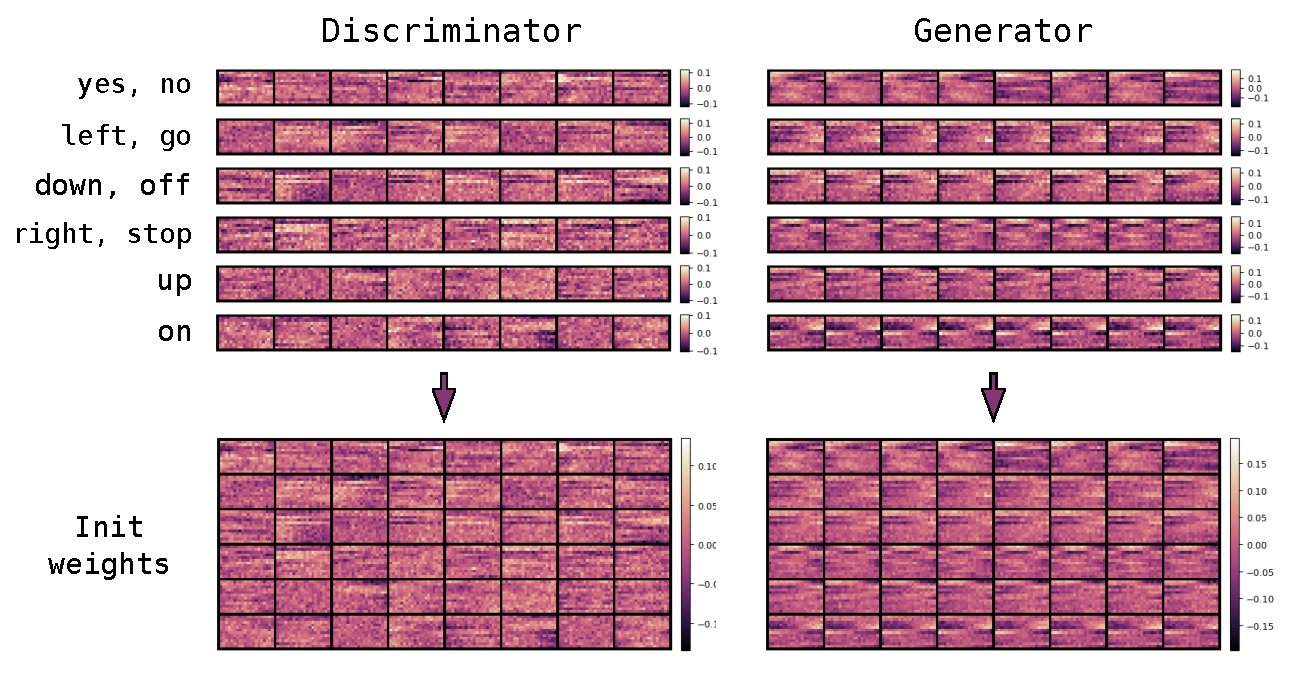
\includegraphics[width=0.7\textwidth]{./4_nn/figs/nn_adv_label_scheme}
  \caption{Label training scheme, trained with 100 epochs for each label subset.}
  \label{fig:nn_adv_label_scheme}
\end{figure}
\FloatBarrier
\noindent


% \subsection{Questions that arise}
% There are several questions that arise regarding Adversarial Training:
% \begin{enumerate}[label={Q.\textgoth{A}.\arabic*)}, leftmargin=1.4cm]
%   \item Does the Network Architecture of G and D have to be the same but transposed?
%   \item Does the value space of in and outputs, for D and G respectively, have to be limited between a range of [0, 1] done by for instance the frame normalization, or sigmoid output?
%   \item What loss function works well for training?
%   \item How long should be trained?
%   \item When transfering weights to another network, should the weights from G or D be transfered?
%   \item Does the classification network has to adapt the parameters from the transfered weights?
%   \item Whats the benefit of all this?
% \end{enumerate}

% To illustrate the idea an example is shown of the labels L5 (left, right, up, down, go).

% The convolutional layer weights from the adversarial training of the individual labels, 
% can be stacked together an used to initialize another network.
% An example of this method is shown in \rfig{nn_adv_example}, where the initialization pattern changes to more elaborate structures and patterns to form good classification outputs. 
% However the Basic Pattern from the adversarial training stays the same, which is a good sign, because then the network is accepting those trained weights and adapts them.

% \begin{figure}[!ht]
%   \centering
%     \subfigure[c1 trained]{\includegraphics[width=0.45\textwidth]{./4_nn/figs/nn_adv_example_c0}}
%     \subfigure[c1 init]{\includegraphics[width=0.45\textwidth]{./4_nn/figs/nn_adv_example_c0_init}}
%     \subfigure[c2 trained]{\includegraphics[height=0.45\textwidth]{./4_nn/figs/nn_adv_example_c1}}
%     \quad
%     \subfigure[c2 init]{\includegraphics[height=0.45\textwidth]{./4_nn/figs/nn_adv_example_c1_init}}
%   \caption{Adversarial Training Example: Convolutional layers pretrained with adversarial training on each label separately.}
%   \label{fig:nn_adv_example}
% \end{figure}
% \FloatBarrier
% \noindent

% For this example in adversarial training, 8 feature maps of the first layer were used for each label, also they belong to the Generator Network G or decoder (dec). In Convolutional Networks, each previous layers feature map creates a new set of feature maps in the next layer.
% An example of this label training is shown in \rfig{nn_adv_example_label} with feature maps [(1, 8), (8, 8)] of the convolutional layers

% \begin{figure}[!ht]
%   \centering
%     \subfigure[\enquote{left} c1 from D]{\includegraphics[width=0.45\textwidth]{./4_nn/figs/nn_adv_example_label_left_c0_enc}}
%     \subfigure[\enquote{left} c1 from G]{\includegraphics[width=0.45\textwidth]{./4_nn/figs/nn_adv_example_label_left_c0_dec}}
%     \subfigure[\enquote{left} c2 from D]{\includegraphics[width=0.3\textwidth]{./4_nn/figs/nn_adv_example_label_left_c1_enc}}
%     \subfigure[\enquote{left} c2 from G]{\includegraphics[width=0.3\textwidth]{./4_nn/figs/nn_adv_example_label_left_c1_dec}}
%   \caption{Adversarial Training example of Generator (G) and Discriminator (D) of label \enquote{left} captured with 8 feature maps of the first convolutional layer.}
%   \label{fig:nn_adv_example_label}
% \end{figure}
% \FloatBarrier
% \noindent

% Those trained weights from each label can then simply be put into the feature maps of a classification network.
% This is shown in \rfig{nn_adv_example} where c1 from G and c2 from G in \rfig{nn_adv_example_label} were transfered to the first row(s).
% When doing the transferring of feature maps, it is important that the layers are not mixed up so that the trained connections are still correct.
% Also of course the weights of the feature maps must have the same dimension, so that transferring is possible.


% \subsection{Observing the Generators output}
% While the output of the Discriminator is rather uninteresting (one-dimensional probability value), the output of the Generator is a good indicator of how well the training between D and G has gone.
% Optimally the output of the Generator look like real data samples.
% An example of a trained Generator Network with fake outputs compared to real ones is shown in \rfig{nn_adv_gen}.

% \begin{figure}[!ht]
%   \centering
%     \subfigure[\enquote{left} real examples]{\includegraphics[width=0.45\textwidth]{./4_nn/figs/nn_adv_gen_left_real}}
%     \subfigure[\enquote{left} fakes from G]{\includegraphics[width=0.45\textwidth]{./4_nn/figs/nn_adv_gen_left_fake}}
%   \caption{Real samples of \enquote{left} from the Speech Commands dataset compared to fake samples from a trained Generator Network.}
%   \label{fig:nn_adv_gen}
% \end{figure}
% \FloatBarrier
% \noindent

% If the fake example of the Generator Network do not look similar to real ones, then something might have gone wrong in the training between the Generator and Discriminator Network.
% Further it can be evaluated if a certain network architecture is able to produce a label in a sufficient representation, therefore this method might be a good start in finding a suitable network architecture for the problem to be solved.



